\documentclass[11pt]{article}
\usepackage{graphicx}    % needed for including graphics e.g. EPS, PS
\topmargin -1.5cm        % read Lamport p.163
\oddsidemargin -0.04cm   % read Lamport p.163
\evensidemargin -0.04cm  % same as oddsidemargin but for left-hand pages
\textwidth 16.59cm
\textheight 21.94cm 
%\pagestyle{empty}       % Uncomment if don't want page numbers
\parskip 7.2pt           % sets spacing between paragraphs
%\renewcommand{\baselinestretch}{1.5} % Uncomment for 1.5 spacing between lines
\parindent 0pt		 % sets leading space for paragraphs

\usepackage{listings}
\usepackage{color}



\begin{document}         


\begin{figure}[htp]
\centering
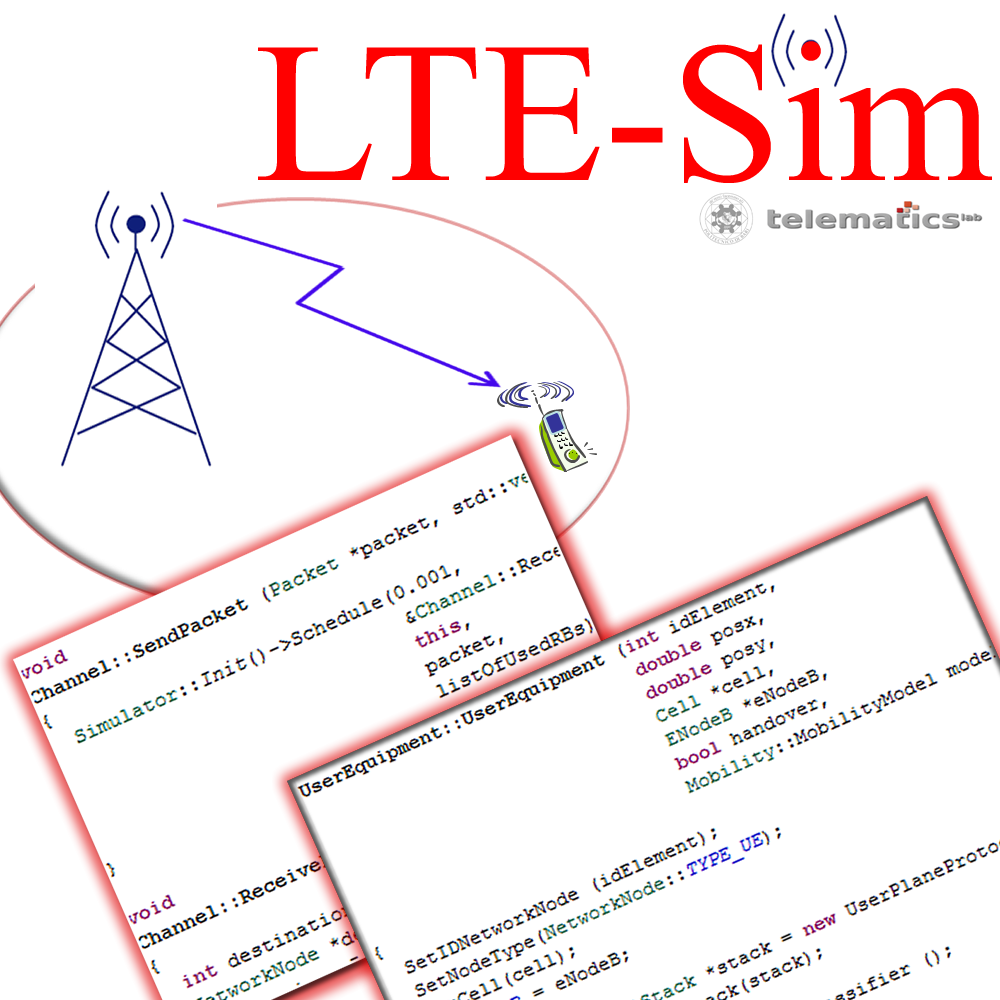
\includegraphics{lte-sim-web.png}
\end{figure}




LTE-Sim is an open source framework to simulate LTE networks.

It encompasses several aspects of LTE networks, including both the Evolved Universal Terrestrial Radio Access (E-UTRAN) and the Evolved Packet System (EPS). It supports single and multi-cell environments, QoS management, multi users environment, user mobility, handover procedures, and frequency reuse techniques. Three kinds of network nodes are modeled: user equipment (UE), evolved Node B (eNB) and Mobility Management Entity/Gateway (MME/GW). Four different traffic generators at the application layer have been implemented and the management of data radio bearer is supported. Finally, well-known scheduling strategies (such as Proportional Fair, Modified Largest Weighted Delay First, and Exponential Proportional Fair), AMC scheme, Channel Quality Indicator feedback, frequency reuse techniques, and models for physical layer have been developed.

The purpose of this tutorial is to make it easier for new users to use LTE-Sim, to create their own simulation scenarios and to eventually add new functionality to LTE-Sim.



\section{Getting LTE-Sim}
LTE-sim is available via Subversion To obtain LTE-Sim, enter into the your preferred folder and
write the following syntax:
\color{blue}
\begin{lstlisting}
$ svn co http://telematics.poliba.it/svn/LTE-Sim 
\end{lstlisting}
\color{black}
To synchronize the project repository with the local copy, you can run update sub-command. The syntax is as follows:
\color{blue}
\begin{lstlisting}
$ svn update
\end{lstlisting}
\color{black}

\section{Compiling LTE-Sim}
On Linux systems, you can buil LTE-Sim with the following command:
\color{blue}
\begin{lstlisting}
$ make
\end{lstlisting}
\color{black}

To clear the project, you can use the following command:
\color{blue}
\begin{lstlisting}
$ make clean
\end{lstlisting}
\color{black}

For both Linux and Windows systems, you can import the LTE-Sim into the your preferred development platform (i.e., eclipse). To this aim, you can create a C++ project and copy/paste all files of LTE-Sim/src into the src folder of your project.  


\section{Running LTE-Sim}
In this release several LTE scenarios have been developed as an example. To run a simple simulation, you can use the following command:
\color{blue}
\begin{lstlisting}
$ ./LTE-Sim Simple
\end{lstlisting}
\color{black}

Using 
\color{blue}
\begin{lstlisting}
$ ./LTE-Sim -h
\end{lstlisting}
\color{black}
you can take a look to LTE scenarios we have developed as an example.


\section{Software Design} \label{design}
\begin{figure}[htp]
\centering
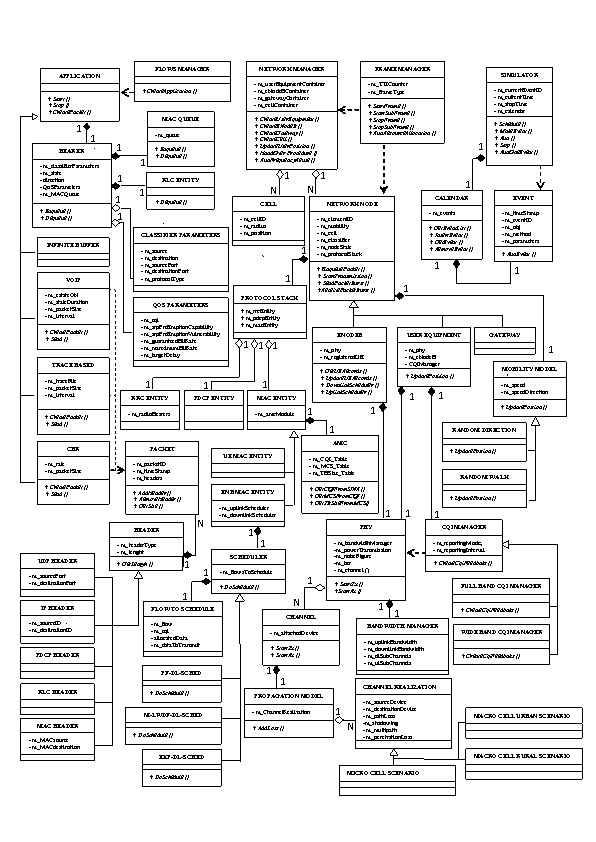
\includegraphics{uml.png}
\caption{LTE-Sim - the class diagram}
\end{figure}


\section{Build a simple scenario} \label{simple-scenario}

With LTE-Sim, a LTE scenario can be created as a static function in a C++ header file, that should be stored into the Simulation/Scenarios folder. A reference of this function should be added into the main program. In this way, the user is able to simulate a proper LTE scenario, selecting it directly from the main program. 

A basic scenario can be created using the following guidelines:
\begin{itemize}
	\item create an instance for \emph{Simulator}, \emph{NetworkManager}, \emph{FlowsManager}, and \emph{FrameManager} components.
	\item Create \emph{Cell}, \emph{ENodeB}, and \emph{UE} objects using methods of the \emph{NetworkManager} class. For each of these objects, several parameters can be assigned directly with the constructor of the class. 
	\item Create applications, defining for each of them the data radio bearer type (GBR or non-GBR), IP classifier parameters, the start time, the stop time, and QoS parameters.
	\item Define the duration of the simulation and, finally, call the \emph{Simulator::Run()} function.  
\end{itemize}

In order to build a simple scenario, the first step is to define a new static function into the src/Simulation/SCENARIOS folder. For this tutorial, we call this function "SimpleScenario", and we define it into the SimpleScenario.h header file. 

\color{blue}
\begin{lstlisting}
#include "../channel/LteChannel.h"
#include "../core/spectrum/bandwidth-manager.h"
#include "../networkTopology/Cell.h"
#include "../core/eventScheduler/simulator.h"
#include "../flows/application/InfiniteBuffer.h"
#include "../flows/QoS/QoSParameters.h"
#include "../componentManagers/FrameManager.h"
#include "../componentManagers/FlowsManager.h"

static void SimpleScenario ()
{
}
\end{lstlisting}
\color{black}

From this point, all instructions must be inserted into the "{}" of the previous declarated static function.

Create four basic LTE-Sim components (the \emph{NetworkManager}, the \emph{FramekManager}, the \emph{FlowManager}, and the \emph{Simulator}).
\color{blue}
\begin{lstlisting}
  Simulator *simulator = Simulator::Init();
  FrameManager *frameManager = FrameManager::Init();
  NetworkManager* networkManager = NetworkManager::Init();
  FlowsManager* flowsManager = FlowsManager::Init ();
\end{lstlisting}
\color{black}
 
Create Channels and Spectrum
\color{blue}
\begin{lstlisting}
  LteChannel *dlCh = new LteChannel ();
  LteChannel *ulCh = new LteChannel ();
  BandwidthManager* spectrum = new BandwidthManager (5, 5, 0, 0);
\end{lstlisting}
\color{black}

Create an LTE cell.
\color{blue}
\begin{lstlisting}
  // CREATE CELL
  int idCell = 0;
  int radius = 1; //km
  int minDistance = 0.0035; //km
  int posX = 0;
  int posY = 0;
  Cell* cell = networkManager->CreateCell (
		idCell, radius, minDistance, posX, posY);
\end{lstlisting}
\color{black}

Create network elements (eNB, GW, and UE).
\color{blue}
\begin{lstlisting}
 //Create ENodeB
  int idEnb = 1;
  ENodeB* enb = networkManager->CreateEnodeb (
		idEnb, cell, posX, posY, dlCh, ulCh, spectrum);
  enb->SetDLScheduler (ENodeB::DLScheduler_TYPE_PROPORTIONAL_FAIR);

  //Create GW
  Gateway *gw = networkManager->CreateGateway ();

  //Create UE
  int idUe = 2;
  int posX_ue = 40; //m
  int posY_ue = 0;  //m
  int speed = 3;    //km/h
  double speeDirection = 0;
  UserEquipment* ue = networkManager->CreateUserEquipment (
		idUe, posX_ue, posY_ue, speed, speeDirection, cell, enb);
\end{lstlisting}
\color{black}



Create an Infinete Buffer Application

\color{blue}
\begin{lstlisting}
  //Create an Application
  QoSParameters *qos = new QoSParameters ();
  int applicationID = 0;
  int srcPort = 0;
  int dstPort = 100;
  int stratTime = 10; //s
  int stopTime = 30;  //s
  Application* be = flowsManager->CreateApplication (
		applicationID,
		gw, ue,
		srcPort, dstPort, TransportProtocol::TRANSPORT_PROTOCOL_TYPE_UDP ,
		Application::APPLICATION_TYPE_INFINITE_BUFFER,
		qos,
		stratTime, stopTime);

\end{lstlisting}
\color{black}

Define the duration of the simulation.
\color{blue}
\begin{lstlisting}
  simulator->SetStop(60);
\end{lstlisting}
\color{black}

Call the \emph{Simulator::Run()} function to strat the simulation.
\color{blue}
\begin{lstlisting}
  simulator->Run ();
\end{lstlisting}
\color{black}

Finally, a reference of SimpleScenario() should be added into the main program. To this aim, insert into the LTE-Sim.cpp main program the folowing code:

\color{blue}
\begin{lstlisting}
#include "Simulations/SCENARIOS/SimpleScenario.h"
int
main (int argc, char *argv[])
{

  ...

	if(strcmp(argv[1], "SimpleScenario")==0)
	  {
   	    SimpleScenario();
	  }
}
\end{lstlisting}
\color{black}



\end{document}
